\documentclass[
	ngerman,
	xcolor=dvipsnames,
	11pt
	]{beamer}
\usepackage{babel}
%\usepackage[T1]{fontenc}
\usepackage[utf8]{inputenc}
%\usepackage{ae}
%\usepackage{lmodern}
\usepackage[T1]{fontenc}
\usepackage[math]{iwona}
%\usepackage{fix-cm}
%\usepackage{epigrafica}
%\usepackage{helvet}
%\usepackage{mathptmx}
%\usepackage{soul}	%\textst command
\usepackage{ulem} 	%\uline \sout \xout \uuline \uwave

\usepackage{tikz}
\usetikzlibrary{arrows,calc}
\tikzset{
%Define standard arrow tip
>=stealth',
%Define style for different line styles
help lines/.style={dashed, thick},
axis/.style={<->},
important line/.style={thick},
connection/.style={thick, dotted},
}

\newcommand{\beginbackup}{
   \newcounter{framenumbervorappendix}
   \setcounter{framenumbervorappendix}{\value{framenumber}}
}
\newcommand{\backupend}{
   \addtocounter{framenumbervorappendix}{-\value{framenumber}}
   \addtocounter{framenumber}{\value{framenumbervorappendix}} 
}

%% outer theme
%\useoutertheme{miniframes}   % Navigation oben
%\useoutertheme{shadow}       % Schatten unter dem frametitle
%\useoutertheme{infolines}
%\useoutertheme{split}        % infolines wie in warsaw

%% inner theme
%\useinnertheme{default}      % dreiecke
%\useinnertheme[shadow=true]{rounded}

%% font theme
%\usefonttheme{structurebold} % dicke Überschriften

%% color theme
% beaver: rot-grau
% crane: sandgelb
% dolphin: hellblau
% orchid: Kasten kräftig
% rose: kasten matt
% seahorse: grau-blau

%\usecolortheme[named=red]{structure}


%\usetheme{Warsaw}
%\usetheme{Boadilla}
%\usetheme{Singapore}
%\usetheme{CambridgeUS}
%\usetheme{Frankfurt}
%\usetheme{Madrid}


%% set templates
%\setbeamertemplate{headline}{}
%\setbeamertemplate{items}[ball]
\setbeamertemplate{navigation symbols}{}

%% Progressbar
%\usetheme{progressbar}
%\usecolortheme{seahorse}
%\setbeamercolor{title page foot}{bg=blue}
%\useoutertheme{progressbar32}
%\progressbaroptions{frametitle=normal,headline=sections,titlepage=normal}
%\setbeamertemplate{background canvas}{}

%% TUBS
\usetheme[pageofpages=von,% page count separator
          tulogo=tubs,
			 institutelogo=ida]
			 {TUBS}
\usecolortheme{tubs}

%% Singapore
%\useoutertheme{infolines}
%\usetheme{Singapore}
%\useinnertheme[shadow=true]{rounded}
%\usecolortheme[named=Gray]{structure}
%\usecolortheme{rose}

%% CambridgeUS
%\useoutertheme{shadow}
%\usetheme{CambridgeUS}
%\useinnertheme[shadow=true]{rounded}
%\usecolortheme[named=darkred]{structure}
%\setbeamertemplate{items}[ball]
%\setbeamertemplate{headline}{}
%\usecolortheme{orchid}

%% Frankfurt
%\usetheme{Frankfurt}
%\useoutertheme{infolines}
%\setbeamertemplate{headline}{}
%\usecolortheme[named=Brown]{structure}

%% Boadilla | Madrid
%\usetheme{Boadilla}
%\usecolortheme[named=Green]{structure}

%% TUBS
%\setbeamercolor{background canvas}{bg=blue}
%\useoutertheme{default}
%\usecolortheme{orchid}

\title[ShortTitle]{Der Konfliktverlauf}
\author{Johannes Schlatow}
\institute{}
\date{\today}

%\AtBeginSubsection[]
%{
%  \begin{frame}<beamer>
%    \frametitle{Layout}
%    \tableofcontents[currentsection,currentsubsection]
%  \end{frame}
%}

\newenvironment{annot}{\begin{block}{}\it}{\end{block}}

\begin{document}

\begin{frame}[t,plain]
	\titlepage
\end{frame}

%\frame{\tableofcontents}
\begin{frame}
	\frametitle{Motivation}
\begin{annot}
	Häufig wird unterbewusst gehandelt. Eine \textbf{Sensibilisierung} für typische Aspekte soll bei der Erkennung und Auflösung von Konflikten helfen.	
\end{annot}

Konflikt\ldots
\begin{description}
	\item \ldots Auslöser
	\item \ldots Symptome
	\item \ldots Ursachen
	\item \ldots Dynamik
\end{description}
\end{frame}

\section{Entstehung}
\subsection{Vom latenten zum manifesten Konflikt}
\begin{frame}
	\frametitle{Vom latenten zum manifesten Konflikt}
%	Existiert der \textbf{plötzliche} Konflikt?

%	\begin{itemize}
%		\item \textbf{latenter} Konflikt
%		\item Konfliktauslöser
%		\item \textbf{manifester} Konflikt
%	\end{itemize}

  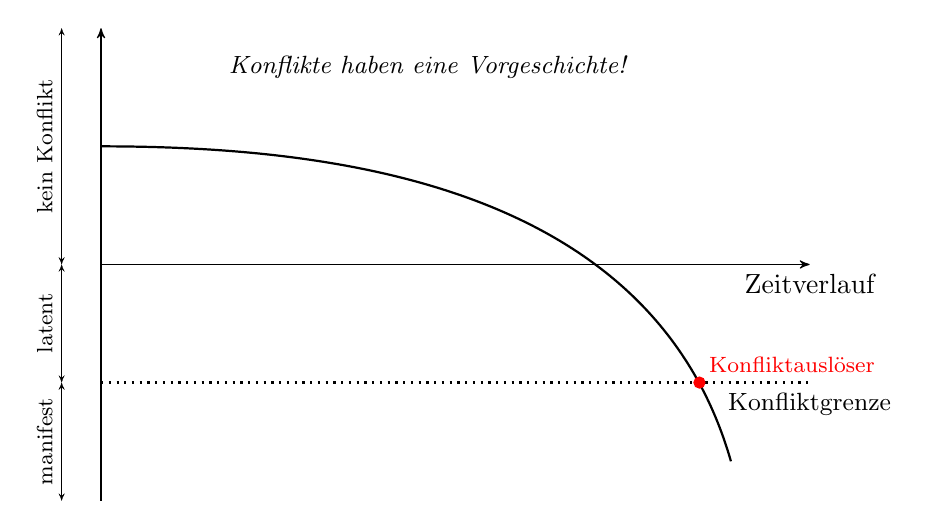
\begin{tikzpicture}[scale=1]
    % Axis
    \coordinate (y) at (0,3);
    \coordinate (x) at (9,0);
	 \draw[<-] (y) -- (0,0) -- (0,-3);
	 \draw[->] (0,0) --  (x) node[below] {Zeitverlauf};
	 % A grid can be useful when defining coordinates
    % \draw[step=1mm, gray, thin] (0,0) grid (5,5); 
    % \draw[step=5mm, black] (0,0) grid (5,5); 

    % Let us define some coordinates
    \path
    coordinate (start) at (0,1.5)
    coordinate (c1) at +(3,1.5)
    coordinate (c2) at +(7,1)
    coordinate (slut) at (8,-2.5);

    \draw[important line] (start) .. controls (c1) and (c2) .. (slut);
	 \draw[connection] (0,-1.5) -- (9,-1.5) node[below] {\small{Konfliktgrenze}};

	 \draw[<->,ultra thin] (-.5,0) -- node[above,sloped] {\footnotesize{kein Konflikt}} (-.5,3);
	 \draw[<->,ultra thin] (-.5,-1.5) -- node[above,sloped] {\footnotesize{latent}} (-.5,0);
	 \draw[<->,ultra thin] (-.5,-3) -- node[above,sloped] {\footnotesize{manifest}} (-.5,-1.5);

	 \draw (1.5,2.5) node [right] {\small{\textit{Konflikte haben eine Vorgeschichte!}}};

    % Help coordinates for drawing the curve
    % \filldraw [black] 
    % (start) circle (2pt)
    % (c1) circle (2pt)
    % (c2) circle (2pt)
    % (slut) circle (2pt)
    \filldraw [red] 
	 (7.6,-1.5) circle (2pt) node[above right, red] {\footnotesize{Konfliktauslöser}};

%     % We start the second graph
%     \begin{scope}[xshift=6cm]
%       % Axis
%      \coordinate (y2) at (0,5);
%      \coordinate (x2) at (5,0);
%      \draw[axis] (y2) node[above] {$r$} -- (0,0) --  (x2) node[right] {$L$};
%      % Define some coodinates
%     \path
%     let
%     \p1=(top)
%     in
%     coordinate (sstart) at (1,.5) 
%     coordinate (sslut) at (4, 4.5)
%     coordinate (dstart) at (4,.5)
%     coordinate (dslut) at (1,4.5)
%% Intersection 1
%     coordinate (int) at  (intersection cs:
%       first line={(sstart)--(sslut)},
%       second line={(dstart)--(dslut)})
%% Intersection 2
%    coordinate (int2) at  (intersection cs:
%       first line={(top)--($(10,\y1)$)},
%       second line={(dstart)--(dslut)})
%% Intersection 3
%    coordinate (int3) at  (intersection cs:
%       first line={(top)--($(10,\y1)$)},
%       second line={(sstart)--(sslut)});
%% Draw the lines
%     \draw[important line] (sstart) -- (sslut) node[above right] {$S$}
%       (dstart) -- (dslut)  node[above left] {$D$};
%     \draw[connection] let \p1=(int2), \p2=(int3) in 
%     (int2)--(\x1,0) node[below] {$\mathit{L_D}$}
%     (int3)--(\x2,0) node[below] {$\mathit{L_S}$};
%      \end{scope}
%%Finally, connect the two graphs
%     \draw[connection] let \p1=(top), \p2=(x2) in (0,\y1) node[left]
%     {$r^*$} -- (\x2, \y1);
    \end{tikzpicture}
	
\end{frame}
\subsection{Konfliktsymptome}
\begin{frame}
	\frametitle{Konfliktsymptome}
	\begin{columns}[t]
		\column{.5\textwidth}
		\begin{block}{Im Gespräch}
			\begin{itemize}
				\item Widerspruch
				\item Desinteresse, Ablenkung
				\item Wiederholung
				\item pauschales ``Ja/Nein''
				\item keine eigenen Vorschläge
				\item offensichtliches Unbehagen
				\item Beschwichtigungfloskeln
			\end{itemize}
		\end{block}
		\pause

		\column{.5\textwidth}
		\begin{block}{Im Verhalten}
			\begin{itemize}
				\item Abweichung vom üblichen
				\item Abspaltung (z.B. Mittagessen)
				\item verminderte Hilfs-/Kooperationsbereitschaft
			\end{itemize}
		\end{block}
	\end{columns}
\end{frame}

\subsection{Regeln in der Entwicklungsphase}
\begin{frame}
	\frametitle{Regeln in der Enwicklungsphase}
	\begin{alertblock}{Keinen Ärger aufstauen}
		Sondern kleine Vorfälle offen ansprechen.\\
		$\Rightarrow$ Konflikte im Keim ersticken!
	\end{alertblock}

	\begin{block}{Konstruktive Kommunikation}
		Sichtweisen der Gegenseite ermitteln
		\begin{description}
			\item \textit{dazu:} offene Fragen stellen
			\item \textit{aber:} Wertung vermeiden
		\end{description}
	\end{block}
\end{frame}

\section{Manifestierung}
\begin{frame}
	\frametitle{Konfliktursachen}

	\begin{itemize}
		\item Subjektive Wichtigkeit entscheidet. \textit{Beispiel: Religion}
		\item Konfliktherd ``Arbeitsplatz''
		\item Menschen sind unterschiedlich
	\end{itemize}

	\hfill
	\pause
	\begin{annot}
		Ursachen (er)kennen, um einen Konflikt zu lösen.
	\end{annot}
\end{frame}

\begin{frame}
	\frametitle{Konfliktarten I}	

	\begin{columns}[t]
		\begin{column}{.5\textwidth}
			\begin{exampleblock}<1->{Beziehungskonflikt}
				Persönliche Abneigungen, Antisympathie
			\end{exampleblock}

			\begin{exampleblock}<2->{Verteilungskonflikt}
				Ungleiche, ungerechte Ressourcenverteilung	
			\end{exampleblock}	
		\end{column}
	
		\begin{column}{.5\textwidth}
			\begin{exampleblock}<3->{Zielkonflikt}
				Beispiel: Berufswahl
			\end{exampleblock}

			\begin{exampleblock}<4->{Beurteilungskonflikt}
				Meinungen über die \textbf{Umsetzung} eines Zieles divergieren.
			\end{exampleblock}
		\end{column}
	\end{columns}
\end{frame}

\begin{frame}
	\frametitle{Konfliktarten II}

	\begin{columns}[c]
		\column{.5\textwidth}
		\begin{exampleblock}<1->{Wertekonflikt}
			Beispiel: Arbeitseinstellung
		\end{exampleblock}

		\begin{exampleblock}<2->{Strukturkonflikt}
			Beispiel: Kundenzuständigkeit im Vertrieb
		\end{exampleblock}

		\column{.5\textwidth}
		\begin{exampleblock}<3->{Rollenkonflikt}
			Gegenläufiges Verhalten z.B. privat $\leftrightarrow$ beruflich
		\end{exampleblock}
	\end{columns}

\end{frame}

\section{Grundmuster}
\begin{frame}
	\frametitle{Warum Konflikte eskalieren}
	\begin{itemize}
		\item Kommunikationsfähigkeit lässt nach
		\item Verallgemeinerung $\Rightarrow$ Ausweitung auf andere Themen
		\item Einbeziehung Dritter
	\end{itemize}
	\pause
	\begin{itemize}
		\item Erwartungshaltung $\Rightarrow$ Selbsterfüllende Prophezeiung
		\item Unterbewusstsein
		\item Kognitive Dissonanz
	\end{itemize}

	\pause
	\begin{alertblock}{Innehalten in der Konfliktdynamik}
		Eine Selbstreflektion kann ein weiteres Eskalieren des Konflikts verhindern.
	\end{alertblock}
\end{frame}

\section{Eskalationsstufen}
\begin{frame}
	\frametitle{Die Hauptphasen der Konflikteskalation}
%\begin{columns}[t]
%	\begin{column}{0.33\textwidth}
		\begin{block}{win-win}
			Einigung durch Selbsthilfe möglich.
		\end{block}\pause
%	\end{column}
%	\begin{column}{0.33\textwidth}
		\begin{block}{win-lose}
			Nur die eigene Seite soll gewinnen. Konfliktlösung benötigt Hilfe von außen.
		\end{block}\pause
%	\end{column}
%	\begin{column}{0.33\textwidth}
		\begin{block}{lose-lose}
			Verluste der Gegenseite werden gegen die eigenen aufgewogen.
		\end{block}
%	\end{column}
%\end{columns}
\end{frame}

\subsection{Die neun Eskalationsstufen}
\begin{frame}
	\frametitle{Die neun Eskalationsstufen - win-win}
\begin{columns}[t]
	\begin{column}{0.33\textwidth}
		\begin{block}{1. Verhärtung}
			\begin{itemize}
				\item Differenzen bewusst
				\item \it z.B. tägliche Streitigkeiten
			\end{itemize}
		\end{block}
	\end{column}
	\pause
	\begin{column}{0.33\textwidth}
		\begin{block}{2. Debatte}
			\begin{itemize}
				\item Polarisation
				\item Recht behalten
				\item kognitive Dissonanz
			\end{itemize}
		\end{block}
	\end{column}
	\pause
	\begin{column}{0.33\textwidth}
		\begin{block}{3. Taten statt Worte}
			\begin{itemize}
				\item Trotzreaktionen
				\item \it z.B. Dienst nach Vorschrift
			\end{itemize}
		\end{block}
	\end{column}
\end{columns}
\end{frame}

\begin{frame}
	\frametitle{Die neun Eskalationsstufen\\win-lose}
\begin{columns}[t]
	\begin{column}{0.33\textwidth}
		\begin{block}{4. Soziale Ausweitung}
			\begin{itemize}
				\item ``Luft machen''
				\item Feindbilder
				\item Selbsterfüllende Prophezeiung
			\end{itemize}
		\end{block}
	\end{column}
	\pause
	\begin{column}{0.33\textwidth}
		\begin{block}{5. Gesichtsverlust}
			\begin{itemize}
				\item Bloßstellen
				\item ``point of no return''
				\item \it z.B. Kündigung androhen
			\end{itemize}
		\end{block}
	\end{column}
	\pause
	\begin{column}{0.33\textwidth}
		\begin{block}{6. Drohstrategien}
			\begin{itemize}
				\item Forderungen, Drohungen
				\item Gegendrohungen
				\item Handlungszwang
			\end{itemize}
		\end{block}
	\end{column}
\end{columns}
\end{frame}

\begin{frame}
	\frametitle{Die neun Eskalationsstufen\\lose-lose}
\begin{columns}[t]
	\begin{column}{0.33\textwidth}
		\begin{block}{7. Begrenzte Vernichtungsschläge}
			\begin{itemize}
				\item Drohungen umsetzen
				\item Schaden zufügen
			\end{itemize}
		\end{block}
	\end{column}
	\pause
	\begin{column}{0.33\textwidth}
		\begin{block}{8. Zersplitterung}
			\begin{itemize}
				\item Steigerund der Angriffe
				\item Zunehmend persönlich
			\end{itemize}
		\end{block}
	\end{column}
	\pause
	\begin{column}{0.33\textwidth}
		\begin{block}{9. Gemeinsam in den Abgrund}
			\begin{itemize}
				\item ``Hauptsache die Gegenseite trifft es härter.''
			\end{itemize}
		\end{block}
	\end{column}
\end{columns}
\end{frame}

%
%\begin{frame}
%  \frametitle{A sample slide}
%
%A displayed formula:
%
%\[
%  \int_{-\infty}^\infty e^{-x^2} \, dx = \sqrt{\pi}
%\]
%
%An itemized list:
%
%\begin{itemize}
%  \item itemized item 1
%  \item itemized item 2
%  \item itemized item 3
%\end{itemize}
%
%\begin{theorem}
%  In a right triangle, the square of hypotenuse equals
%  the sum of squares of two other sides.
%\end{theorem}	
%\end{frame}
%
%\begin{frame}
%	\begin{block}
%		Das ist ein Block.
%	\end{block}
%
%	\begin{alertblock}
%		Das ist ein wichtiger Block.
%	\end{alertblock}
%
%	\begin{example}
%		Das ist ein Beispiel
%	\end{example}
%
%\end{frame}


\beginbackup
\begin{frame}
	\frametitle{Tipps zur Selbsthilfe}
	\begin{itemize}
		\item Zuhören
		\item Kritik nicht persönlich nehmen, sondern verhaltensbezogen
		\item Kritik zur Selbstreflektion nutzen
		\item Nicht vorschnell reagieren, Bedenkzeit ansprechen
		\item ``Ausgleichende'' Gegenkritik vermeiden
		\item \sout{``Ja, aber\ldots''} $\Rightarrow$ ``Ja, und\ldots''
	\end{itemize}	
\end{frame}

\begin{frame}
	\frametitle{Kritik äußernd}
	\begin{itemize}
		\item Frühzeitig ansprechen
		\item Fokus auf die spezifische Situation, keine Verallgemeinerung!
		\item Konkretes Fehlverhalten \textbf{wertfrei} beschreiben
		\item Ich-Form $\Rightarrow$ subjektive Äußerung
		\item Du-Form vermeiden $\Rightarrow$ Vorwurfshaltung
		\item Erwartungen, Wünsche, Anregungen formulieren
	\end{itemize}
\end{frame}
\backupend

\end{document}
